\def\baselinestretch{1}
\chapter{CONCLUSION AND FUTHER WORK}
\label{chap:con}
\graphicspath{{Conclusions/ConclusionsFigs/EPS/}{Conclusions/ConclusionsFigs/}}


\def\baselinestretch{1.66}

\section{Conclusion}

Based on the idea of biology research, we implemented an new motion synthesis framework.
We also introduce new mathematical tools for both the graphic motion synthesis research and biological motor control research.
by the idea of topology conjungacy, we unified the different biological idea.

our idea propose an computational efficient method for graphic research.

by the topolgy and symmery property,
the dynamic of system can be catagloryed.





The primary goal of this research is to develop a new motion synthesis method that can get rid of serious constraints of memory cost or computational cost of current \cms paradigms.

The principle contribution of this research is the dynamic understanding of the biological idea of motion primitive.
Motion Primitives are not simply a class of stereotype motion trajectories, underneath supperficail observed stereotype of motions and nerual signals, there lies a deep and important dynamic reason.
Biological motor control strategy doesn't take the trajecotry as the only control object,  also take the stability into consideration.
For the success of motion tasks, motion trajecotry should move in the neighboorhood of attractors of dynamic system.
And the robust of motion control reflects the ability of the dynamic system maintain its qualitative properties, structual stability.


This idea provides an pausible answer for the computational task puzzle.
Because of the robustity of motion primitives, qualitative properties are automatically maintained.
No Control effort is needed for stability of motion.


The idea  structural stability help us to understand morphylogy of motion.
Follow the morphological computationa idea, sturcutral stability comes not from the control, it comes the body and environment.
In a certain situation, motion primtives and their connectivity can be identified by investigating the landscape of the phase portrait of the intrinsic dynamic system.
This idea propose an different idea about relatioship between motion, morphyology and environemnt.

Exploring intrinic dynamic properties is important for both motor control and \cms.
When  intrinsic properties of natural dynamics are explored, motion cotnrol achieved its energy efficiency and \cms achieve natural looking features.






Based on structual stability of primitives, new motion control method are developed.
Motion trajectory is not the concern of motor control, the dynamic system underline are changed in a unified manner that keeps the qualitative properties untouched.
To this ends, the mathematical concept topology conjungacy are introduced.
For involulatray motion adaption, entraintment method are adopted to maintain the topology of a limit cycle.
For volunatry motion adaptation, the effects of control effort is making the original system undergoes a lie group transformation.
Both method maintains the qualitative properties of original dynamic system.




When shaping the dynamics, the basin of attraction is modified in an controlled way.

These two strategy close related to  the biological results.
Entrainment may model the biological center pattern generator, which exist in the spine cord in many verbrate.
While idea of lie group action has close realtionship to the vision system, maybe a model for control effects of vision system.
Thus based on the , a new control framework for motor control is proposed.
The low level controller(\cpg) maintain the stability or qualitative property.
While high level controller(the vision cortex) control the precision or quantative properties of motion.


New control methods are applied to synthesis a various types of motions including walking, balancing and object manipulation.
Different motion style are generated automatically without complex computation.
Also the transformation method is easy to use, many properties can be changed by simply adjust by one parameters.
Different transformation can be applied independently.












 




\section{Futher Work}
Motor Invariant Theory is not an improvement of already \cms techniques, it is a different paradigms.
Research in this theis does expore the implication of the new idea.
For the new idea, there are rooms to improvement, new direction to attack old problems and even new questions,
which worth further research effort.
In this section, we dicusss several potential topics that may interest computer graphic community or biological research.

\subsection{Stability Of Motion Primitives}

Research in this thesis start from   unstable system,  stability are enhanced by adding control effort.
For some motion tasks, it is impossible to model all the control effort that boost the stability.
It is also possible to start from a stable dyanmic system, and deform the phase portrait to make it have a similar shape to the real system.
Such methods may lots details of accuracy but provides better stability and controllability. 

This is very helpful for games or film application.
Physicall realistic is not the only requirement for application purpose.
Animator requires controlbility and stability over physically accurate.
For characters performance acrobate, the characters must not fall even fall is more physically pausible.




\subsection{More Type Of Symmetry}
More type of symmetry will generate more type of transformation that apply to the adapt motion.
All the symmetry applied in this research are linear, which are easy to compute but also very limited.
Exploring more types of symmetry may provides a different adaptation of scheme.
\begin{itemize}

\HiItem{Discrete Symmetry Properties}
Only biedal waking motion are synthesized in this research, an interesting idea is four or more legs motion can be buitl based on the bipedal walking strategy.

This can be done by exploring another type of symmetry: discrete symmetry.
For  example, when the house hound, the hind leg and font leg will move in synchronize or antiphase.




\HiItem{Nonlinear Symmetry from Structual Parameter Turnning}
Nonline symmetry perserving transformation will generate more type of adaptation.
Since nonliner transformation are more tricky to find, it is questionalable how the biological system find it and apply it for motion adaptation.
But nonlinear transformation is suitable for modeling the tranformation  results from the changing system parameters.
For the idea of structural stability we know the results of chaning parameters is equivalnet to have a one one mapping tranformation.
Work out such transformatins directly or approximately may provide a method for motion retargeting.

\HiItem{Symmetry of Partial Differential System}

All the methods developed here are based on the theory of oridinaly differential equation, which is good enough for rigid body dynamics.
In fact the topological property and symmetrical property also commonly exists in partial differential system.
For example of lorenz transformation and maxwell equation.

Symmetrical of Partial differential equations are important for they may extend the control strategy for rigid body dynamcis to control the motion elastic body or locomotion in fluid.

Such motion are more expensive are little addressed by current \cms methods.


\end{itemize}

To exploring more types of symmetry, reformulation the form of equation may easy the task.
Current dynamic equations are based a fix coordinates frame.
It is helpful to formulate the equations in the coordinate free manner or in the local frame.






\subsection{Retargeting Motion Capture Data}
For computer animation, even methods for simulation high dimentional characters are proposed, it is may not be proper to enerate every details by dynamic methods.
An alternative method is use dynamic simulation to modify motion captue data, which is well addressed in many research in computer graphic community.



Based on the idea of topological equivalance, 
motion primitive of different persons or motions of different situation should have the property of topological equivalent.
In state space, there should exist a one to one mapping transformation function.
Motion Data can be transformed into the state space and apply  transformation.


We can use the low dimentional model to find the one to one mapping relationship.
Maybe this method will genereate physically realistic dynamic motion retargeting.





\subsection{Transform and Muscle Actuation}

In the thesis, control effort are applied directly to ensure tranformation.
In biological research, this process is not that direct.
Control effort are generated by the muscle system.


The question muscle actuation is untouched in this research, but look in details, this method also provides an alternative idea of muscle action.
Control effort are applied to transform the dynamic system, muscles can be actuated not by caculation the force but rather directly from the transformation needed.
In certain situation, the idea of transformation will make muscle control more easily.




For the simple  mass spring system.
offset can implemented by chaning the rest length $d$.
speed action can be implemented by chaning the stiffness $K$.
and energy scaling can be achieved by ajust the stiffness $K$ and then restore it.
 

The reason is transformaton can be achieved by two methods.
Either control effort or by chaning the system parameters.

For biological system, the chaning parameters method may be better for it will help motor control system get rid of the necessary feedback and computation. 
In fact most of control effort in the thesis are potential shaping, which only involves of modifty the potential energy.
If muscles are modeled as spring, then poential energy shaping can also achieved through modifiying spring parameters.

This idea may propose an conjuecture for further biological research.
For graphic research, incoporating muscles in this manner will have no effects on motion synthesis or computational work.
The only pontential benifits is that the parameters of mucles can effect the skin deformation.



\subsection{Perception based Dynamics}
Motion perception is an high level capacity, basecall it is based up our object recoganition ability and our dynamic reasoning ability.
When dynamic motion synthesis, we also touch the question of dynamic perception and encoding problem in intelligence.
The topological equivalency and symmery may also provides an understanding of the perception problem.

Based on the idea of topology equivalency,
Neural system may not need to encode the details of dynamic system, neural system can form an analous dynamic system in our brain that is analogys to the real dynamics.
Such model will lack the details accuracy, but get the qualitatives properties right.

Based on the idea of symmetry,
Neural system may store some experience and the symmetrical proeprty of dynamics in memory.
When we see new motion, we may judge the dynamics validity by transform our experience to match observation.


we are not still not sure which method is better, but both of them are better than building a symbolic equation solving the differential equaiton in our brain.
We proprose maybe a new dynamic simulator can be designed based on or test this principles.
Instead following current paradigms in physical simulaltion, where dynamic model are developed first integrate it to get a moition.

Dynamic simullator can be build upton the topology and the symmetrial property.
Animator can specifiy animation by specify its region on phase portraint and how much transforamtion is applied.
If the hypothesis is true, even the method will generate physically inaccurate results, audience will not notice it.

\subsection{Rethink abouth the uncanny valley}
In \cms research, uncanny valley is a challenging phonomenon of perception at the  central. 
When the characters are becomming more and more realistic, there is a big drop in the perception of likeness.
Only over the valley, perception likeness start to increase;
At currently, little is known about overcomming the phenomenon.
mainly because the mechanism behind such phenonemon is unclear.
At the end of the the thesis, a conjecture is propopsed by extending the idea of motor invariant theory.
Figure~\ref{fig:uncannyValley}.

\begin{figure}[!htbp]
  \begin{center}
      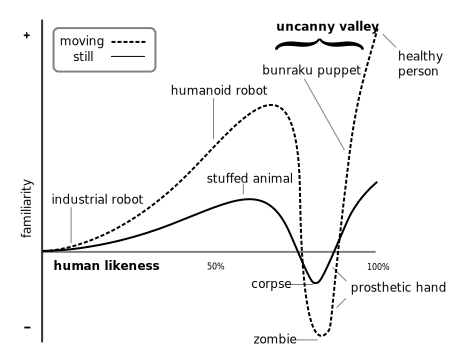
\includegraphics[width=0.5\textwidth]{Mori_Uncanny_Valley}
    \caption{Uncanny Valley}
    \label{fig:uncannyValley}
\end{center}
\end{figure}

The reason behind the uncanny valley is a  a switch of perception mechanism.
For the unfamiliar, the perception mechanism is based on analogy,
where the the identification of qualitative properties plays the major role.
As long as the qualitative properties is the the same with our experience, we may accept them ``belieable''.
This close related to the idea of Global Motor Invariant.

When the object of perception becomes more familiar, 
maybe the quantative details are utilized to match the observation with memory,
which closely relate to the idea of Local Motor Invariant.


A object that have desired qualitative property may not have the quantatative details for quantative mechanism.
When the switch of mechanism results in a drop in likeness.
This proposal is bold and early, but might be a worthwhile topic for further biological and phycological research.





%%% ----------------------------------------------------------------------

% ------------------------------------------------------------------------

%%% Local Variables: 
%%% mode: latex
%%% TeX-master: "../thesis"
%%% End: 
